\begin{frame}[label=overlap_stats]
    \frametitle{Results: Consistent Sampling}
    \begin{center}
        {\colorbox{yellow}{\textbf{Having all \textcolor{red}{\textbf{RX}} within 1.8 km ensures consistent spatial sampling}}}
        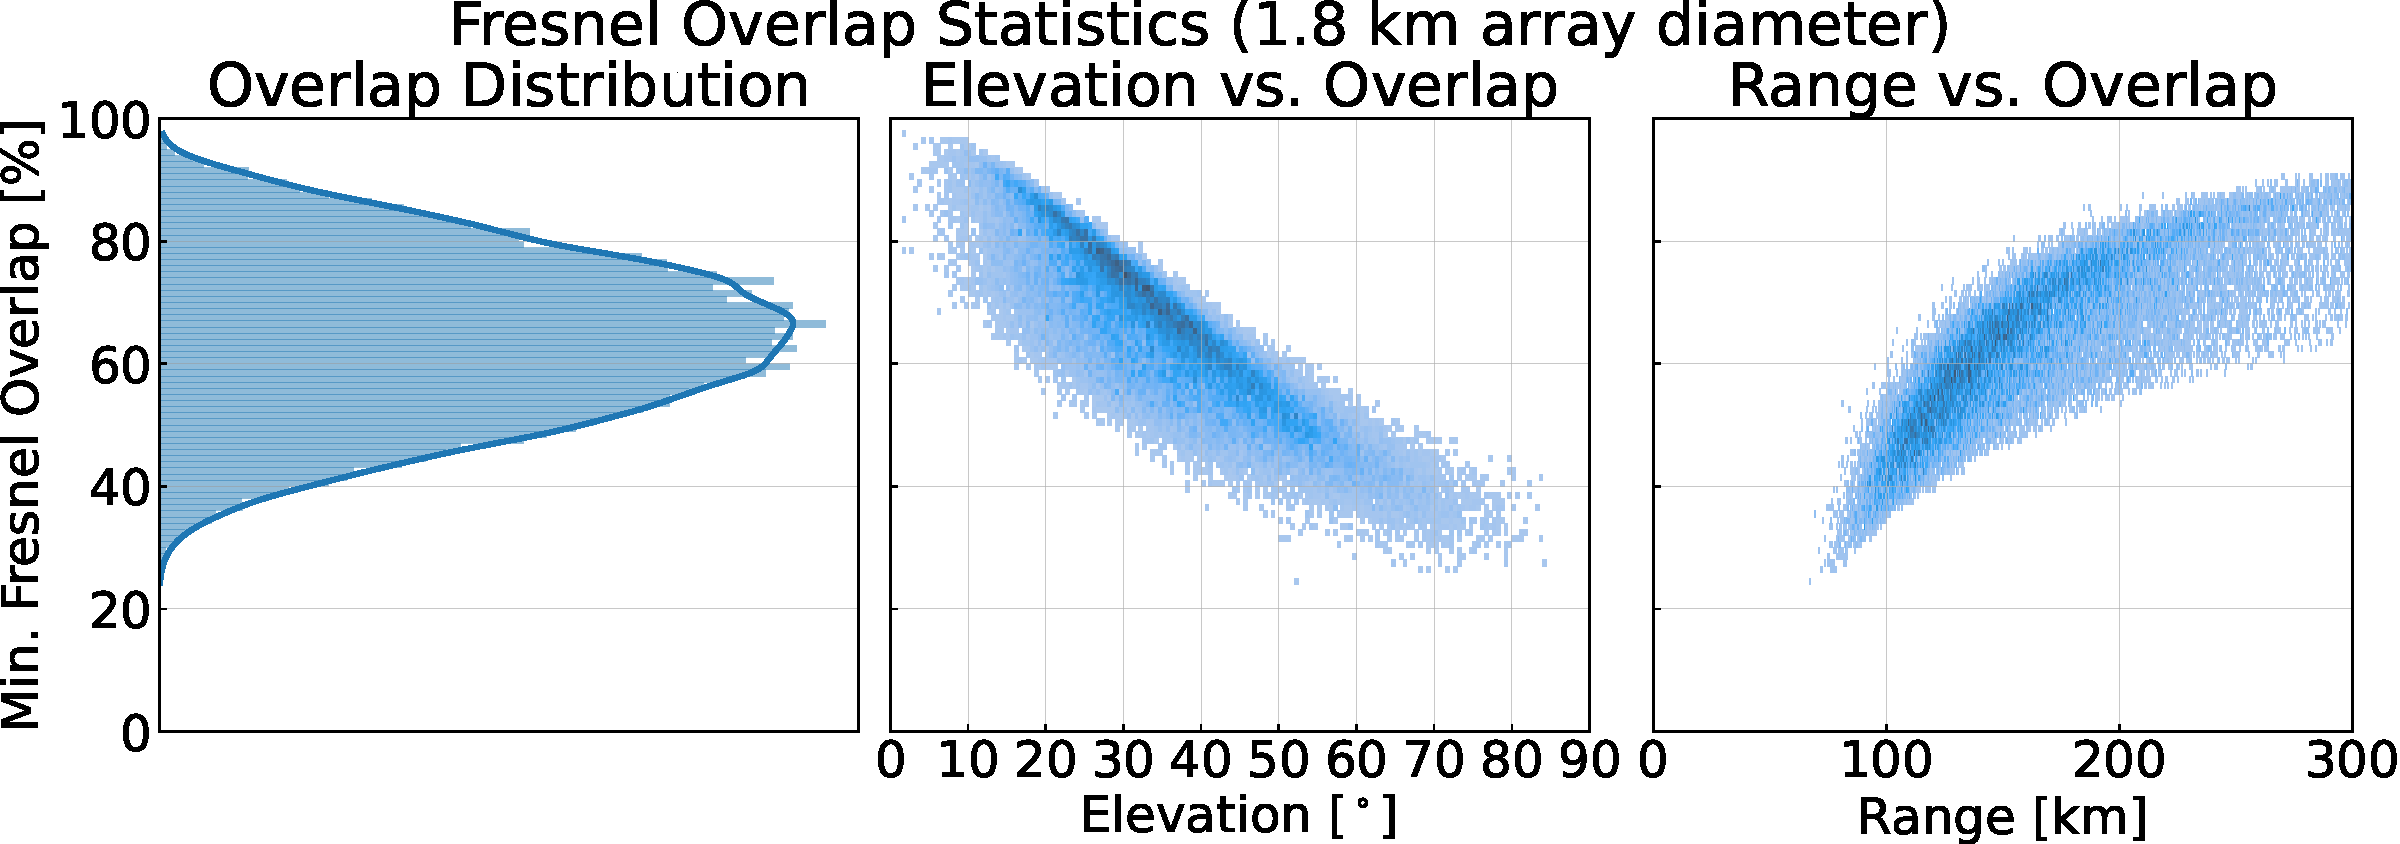
\includegraphics[width=0.8\linewidth]{img/overlap_stats.pdf}
        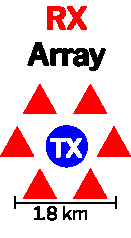
\includegraphics[height=0.35\textheight]{img/rx_array.pdf}
    \end{center}
    \begin{itemize}
        \item[$\blacktriangleright$] \alert{Most meteors seen by all \textcolor{red}{\textbf{RX}}s}: 95\% observations shared by all array members
        \item[$\blacktriangleright$] \alert{Significant Fresnel overlap} 
        \begin{itemize}
            \item 95\% of common observations have >42.9\% overlap
            \item 85\% of common observations have >50\% overlap
        \end{itemize}
    \end{itemize}
\end{frame}